\documentclass{beamer}
\usepackage{uibkstyle}
\usepackage[utf8]{inputenc}
\usepackage[german]{babel}
\usepackage{graphicx}
\usepackage{subfigure}

\usepackage{tikz}
\usetikzlibrary{decorations.pathmorphing}

\graphicspath{{images/}}

\tikzset{
    onslide/.code args={<#1>#2}{%
        \only<#1>{\pgfkeysalso{#2}}
    },
    month/.style={%
        text depth=.25ex,
        text centered,
    }
}
\tikzset{
    other/.style={circle, onslide=<3-7>{white}}
}

\usetikzlibrary{positioning, arrows, decorations.markings}
\tikzset{%label colors for port states
    port/.style={draw, circle},
    dedicated/.style={port, fill=blue!50},
    root/.style={port, fill=green!50},
    blocking/.style={port, fill=red!50}
}

\tikzset{%used for "invisible" stuff
    invisible/.style={draw=white}
    visible/.style={draw=black}
}

\newcommand{\switch}[2]{
    \scalebox{#1}{
        \begin{tikzpicture}
            \node at (0,0) {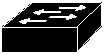
\includegraphics{switch.pdf}};
            \node at (0,-0.6) {#2};
        \end{tikzpicture}
    }
}


\title{STPViz}
\subtitle{Visualizing network topologies with the help of the Spanning Tree Protocol}
\author{Alexander Schlögl}

\begin{document}
\begin{frame}[plain]
    \maketitle
\end{frame}

\begin{frame}{Überblick}
    \begin{itemize}
        \item \textbf{Einleitung \& Motivation}
        \item \textbf{Spanning Tree Protocol (STP)}
        \item \textbf{STPViz}
        \item \textbf{Software-Switch}
        \item \textbf{Tests}
        \item \textbf{Zusammenfassung \& Ausblick}
    \end{itemize}
\end{frame}

\begin{frame}{Überblick}
    \begin{itemize}
        \item \alert{\textbf{Einleitung \& Motivation}}
        \item \textbf{Spanning Tree Protocol (STP)}
        \item \textbf{STPViz}
        \item \textbf{Software-Switch}
        \item \textbf{Tests}
        \item \textbf{Zusammenfassung \& Ausblick}
    \end{itemize}
\end{frame}

\begin{frame}{Einleitung \& Motivation}
    \begin{itemize}
        \item Warum STP?
        \item Was ist das Problem?
        \item Was macht STPViz besser/einfacher?
    \end{itemize}
\end{frame}

\begin{frame}{Warum STP?}
    \begin{itemize}[<+->]
        \item Redundanz in großen Netzwerken erwünscht
        \item Schleifen im Netzwerk entstehen
        \item Das führt zu Broadcast Storms
    \end{itemize}
\end{frame}

\begin{frame}{Broadcast Storms}
    \centering
    \begin{figure}
        \begin{tikzpicture}
            \node (root) at (4,8) {\switch{0.8}{A}};
            \node (B) at (2,6) {\switch{0.8}{B}};
            \node (C) at (6,6) {\switch{0.8}{C}};
            \node (D) at (4,4) {\switch{0.8}{D}};

            \draw
            [onslide=<2>{green, thick, ->},
            onslide=<4>{green,thick, <-},
            onslide=<5>{red,thick,<->}]
            (root) edge (B);

            \draw
            [onslide=<2>{green, thick, ->},
            onslide=<4>{green,thick, <-},
            onslide=<5>{red,thick,<->}]
            (root) edge (C);

            \draw
            [onslide=<3>{red, thick, <->},
            onslide=<5>{red, thick, <->}]
            (B) edge (C);

            \draw
            [onslide=<3>{green, thick, ->},
            onslide=<4-5>{red,thick,<->}]
            (B) edge (D);

            \draw
            [onslide=<3>{green, thick, ->},
            onslide=<4-5>{red,thick,<->}]
            (C) edge (D);
        \end{tikzpicture}
    \end{figure}
\end{frame}

\begin{frame}{Broadcasts mit STP}
    \centering
    \begin{figure}
        \begin{tikzpicture}
            \node (root) at (4,8) {\switch{0.8}{A}};
            \node (B) at (2,6) {\switch{0.8}{B}};
            \node (C) at (6,6) {\switch{0.8}{C}};
            \node (D) at (4,4) {\switch{0.8}{D}};

            \draw
            [onslide=<2>{green,thick,->}]
            (root) edge (B);

            \draw
            [onslide=<2>{green,thick,->}]
            (root) edge (C);

            \draw
            [onslide=<3>{green,thick,->}]
            (B) edge (D);
        \end{tikzpicture}
    \end{figure}
\end{frame}

\begin{frame}{Was sind die Probleme?}
    \begin{itemize}[<+->]
        \item Große Netzwerke sind schwer zu administrieren
        \item STP verbirgt Fehler und Änderungen zusätzlich
        \item STP Konfiguration ist komplex
    \end{itemize}
\end{frame}


\begin{frame}{Was waren unsere Ziele?}
    \begin{itemize}
        \item Nur STP
        \item Geringe verursachte Netzwerkauslastung
        \item Passiv
        \item Verteilt
        \item Geringe Hardwareauslastung
        \item Keine Instandhaltung notwendig
        \item Mehrere Bäume möglich
    \end{itemize}
\end{frame}

\begin{frame}{Zeitplanung}
    \centering
    \begin{figure}
        \begin{tikzpicture}[month]
            \draw (0,0) -- (0.4,0);
            \draw[->] (0.6,0) -- (10,0);
            %cut marker
            \draw[decorate, decoration={snake,amplitude=1pt,segment length=5pt}] (0.41, 0.3) -- (0.41, -0.3);
            \draw[decorate, decoration={snake,amplitude=1pt,segment length=5pt}] (0.62, 0.3) -- (0.62, -0.3);
            \foreach \x in {0,...,9}
                \draw (\x,0.1) -- (\x,-0.1);

            \node at (0,-0.5) {\tiny Oktober};
            \node at (1,-0.5) {\tiny Februar};
            \node at (2,-0.5) {\tiny März};
            \node at (3,-0.5) {\tiny April};
            \node at (4,-0.5) {\tiny Mai};
            \node at (5,-0.5) {\tiny Juni};
            \node at (6,-0.5) {\tiny Juli};
            \node at (7,-0.5) {\tiny August};
            \node at (8,-0.5) {\tiny September};
            \node at (9,-0.5) {\tiny Oktober};

            \draw (0,0.7) rectangle (1,0.5);\node () at (0.5,1) {\tiny Vorarbeit}; 
            \draw (1,0.7) rectangle (3,0.5);\node () at (2,1) {\tiny Implementation}; 
            \draw (3,0.7) rectangle (3.5,0.5);\node () at (3.25,1) {\tiny Tests};
            \draw (3.5,0.7) rectangle (4.5,0.5);\node () at (4,1) {\tiny Zus. Feat.}; 
            \draw (4.5,0.7) rectangle (5,0.5);\node () at (4.75,1) {\tiny Tests};
            \draw (5,0.7) rectangle (6,0.5);\node () at (5.5,1) {\tiny Arbeit}; 
            \draw[->] (6,1.5) -- (6,0);\node () at (6,1.7) {\tiny Presentation};
        \end{tikzpicture}
    \end{figure}
\end{frame}

\begin{frame}{Überblick}
    \begin{itemize}
        \item \textbf{Einleitung \& Motivation}
        \item \alert{\textbf{Spanning Tree Protocol (STP)}}
        \item \textbf{STPViz}
        \item \textbf{Software-Switch}
        \item \textbf{Tests}
        \item \textbf{Zusammenfassung \& Ausblick}
    \end{itemize}
\end{frame}

\begin{frame}{Spanning Tree Protocol}
    \begin{itemize}
        \item Funktionsweise
        \item Pakete
    \end{itemize}
\end{frame}

\begin{frame}{STP Funktionsweise}
    Ports zu doppelten Verbindungen werden deaktiviert.\\
    Für jede Verbindung gibt es genau einen aktiven Port.
    \pause
    \begin{figure}
        \begin{tikzpicture}
            \node (root) at (2,2) {\switch{0.8}{Root}};
            \node (a) at (0,0) {\switch{0.8}{A}};
            \node (b) at (4,0) {\switch{0.8}{B}};

            \draw
            (root) -- node[dedicated, at start]{} node[root, at end]{} (a)
            (root) -- node[dedicated, at start]{} node[root, at end]{} (b)
            (a) -- node[dedicated, at start]{} node[blocking, at end]{} (b);

            \begin{customlegend}[legend cell align=left, legend entries={Root Port,Dedicated Port,Blocking Port},
                legend image post style={scale=2.3},
                legend style={at={(8,2)},font=\footnotesize}]
                \addlegendimage{white,mark=*,fill=green}
                \addlegendimage{white,mark=*,fill=blue!80}
                \addlegendimage{white,mark=*,fill=red}
            \end{customlegend}
        \end{tikzpicture}
    \end{figure}
    \pause
    \footnotesize Bemerkung: Wir werden Switches Bridges nennen
\end{frame}

\begin{frame}{STP Pakete}
    \centering
    \begin{figure}
        \begin{tikzpicture}[scale=0.35]
            \foreach \x in {0,...,31}
            \node at (\x+0.5,20.5) {\scriptsize \x};
            \draw (0,20) rectangle (16,18.5); \node (mode) at (8, 19.25) {Protocol Identifier};
            \draw (16,20) rectangle (24,18.5); \node (mode) at (20, 19.25) {Version Id};
            \draw (24,20) rectangle (32,18.5); \node (mode) at (28, 19.25) {BPDU Type};
            \draw[onslide=<2>{red,line width=3pt}] (0,18.5) rectangle (8,17); \node (mode) at (4, 17.75) {Flags};
            \draw[onslide=<3>{red,line width=3pt}] (8,18.5) rectangle (32,17); \node (mode) at (20, 17.75) {Root Identifier};
            \draw[onslide=<3>{red,line width=3pt}] (0,17) rectangle (32,15.5); \node (mode) at (16, 16.25) {Root Identifier};
            \draw[onslide=<3>{red,line width=3pt}] (0,15.5) rectangle (8,14); \node (mode) at (4, 14.75) {Root Identifier};
            \draw[onslide=<4>{red,line width=3pt}] (8,15.5) rectangle (32,14); \node (mode) at (20, 14.75) {Root Path Cost};
            \draw[onslide=<4>{red,line width=3pt}] (0,14) rectangle (8,12.5); \node (mode) at (4, 13.25) {Root Path Cost};
            \draw[onslide=<5>{red,line width=3pt}] (8,14) rectangle (32,12.5); \node (mode) at (20, 13.25) {Bridge Identifier};
            \draw[onslide=<5>{red,line width=3pt}] (0,12.5) rectangle (32,11); \node (mode) at (16, 11.75) {Bridge Identifier};
            \draw[onslide=<5>{red,line width=3pt}] (0,11) rectangle (8,9.5); \node (mode) at (4, 10.25) {Bridge Identifier};
            \draw (8,11) rectangle (24,9.5); \node (mode) at (16, 10.25) {Port Identifier};
            \draw[onslide=<6>{red,line width=3pt}] (24,11) rectangle (32,9.5); \node (mode) at (28, 10.25) {Message Age};
            \draw[onslide=<6>{red,line width=3pt}] (0,9.5) rectangle (8,8); \node (mode) at (4, 8.75) {Message Age};
            \draw (8,9.5) rectangle (24,8); \node (mode) at (16, 8.75) {Max Age};
            \draw (24,11) rectangle (32,8); \node (mode) at (28, 8.75) {Hello Time};
            \draw (0,8) rectangle (8,6.5); \node (mode) at (4, 7.25) {Hello Time};
            \draw (8,8) rectangle (24,6.5); \node (mode) at (16, 7.25) {Forward Delay};
        \end{tikzpicture}
    \end{figure}
\end{frame}

\begin{frame}{Überblick}
    \begin{itemize}
        \item \textbf{Einleitung \& Motivation}
        \item \textbf{Spanning Tree Protocol (STP)}
        \item \alert{\textbf{STPViz}}
        \item \textbf{Software-Switch}
        \item \textbf{Tests}
        \item \textbf{Zusammenfassung \& Ausblick}
    \end{itemize}
\end{frame}

\begin{frame}{STPViz}
    \begin{itemize}
        \item Struktur \& Funktionsweise
        \item Probleme
        \item Fehlerkorrektur
        \item Darstellung
    \end{itemize}
\end{frame}

\begin{frame}{Struktur \& Funktion}
    \begin{itemize}[<+->]
        \item Mehrere Clients senden ihre Daten an einen Server.
        \item Server kombiniert Daten.
        \item Parser erstellt Visualisierung
    \end{itemize}
    \pause
    Client sammelt Daten aus STP Paketen und kombiniert sie zu einem Pfad zur Root.
\end{frame}

\begin{frame}{STP Pakete}
    \centering
    \begin{figure}
        \begin{tikzpicture}[scale=0.35]
            \foreach \x in {0,...,31}
            \node at (\x+0.5,20.5) {\scriptsize \x};
            \draw (0,20) rectangle (16,18.5); \node (mode) at (8, 19.25) {Protocol Identifier};
            \draw (16,20) rectangle (24,18.5); \node (mode) at (20, 19.25) {Version Id};
            \draw (24,20) rectangle (32,18.5); \node (mode) at (28, 19.25) {BPDU Type};
            \draw (0,18.5) rectangle (8,17); \node (mode) at (4, 17.75) {Flags};
            \draw[red, line width=2pt] (8,18.5) rectangle (32,17); \node (mode) at (20, 17.75) {Root Identifier};
            \draw[red, line width=2pt] (0,17) rectangle (32,15.5); \node (mode) at (16, 16.25) {Root Identifier};
            \draw[red, line width=2pt] (0,15.5) rectangle (8,14); \node (mode) at (4, 14.75) {Root Identifier};
            \draw (8,15.5) rectangle (32,14); \node (mode) at (20, 14.75) {Root Path Cost};
            \draw (0,14) rectangle (8,12.5); \node (mode) at (4, 13.25) {Root Path Cost};
            \draw[blue, line width=2pt] (8,14) rectangle (32,12.5); \node (mode) at (20, 13.25) {Bridge Identifier};
            \draw[blue, line width=2pt] (0,12.5) rectangle (32,11); \node (mode) at (16, 11.75) {Bridge Identifier};
            \draw[blue, line width=2pt] (0,11) rectangle (8,9.5); \node (mode) at (4, 10.25) {Bridge Identifier};
            \draw (8,11) rectangle (24,9.5); \node (mode) at (16, 10.25) {Port Identifier};
            \draw[green, line width=2pt] (24,11) rectangle (32,9.5); \node (mode) at (28, 10.25) {Message Age};
            \draw[green, line width=2pt] (0,9.5) rectangle (8,8); \node (mode) at (4, 8.75) {Message Age};
            \draw (8,9.5) rectangle (24,8); \node (mode) at (16, 8.75) {Max Age};
            \draw (24,11) rectangle (32,8); \node (mode) at (28, 8.75) {Hello Time};
            \draw (0,8) rectangle (8,6.5); \node (mode) at (4, 7.25) {Hello Time};
            \draw (8,8) rectangle (24,6.5); \node (mode) at (16, 7.25) {Forward Delay};
        \end{tikzpicture}
    \end{figure}
\end{frame}

\begin{frame}{Pfadkonstruktion}
    \centering
    \begin{figure}
        \begin{tikzpicture}[nodes=draw]
            \node[circle, red, onslide=<4-6>{white},onslide=<8>{red}] (r) at (16,10) {};

            \node[circle,onslide=<3-5>{white},onslide=<6>{red}] (a0) at (13, 9) {};
            \node[other] (a1) at (15.5, 9) {};
            \node[other] (a2) at (18, 9) {};

            \node[other] (b0) at (12, 8) {};
            \node[circle,onslide=<3-4>{white},onslide=<5>{red}] (b1) at (13.7, 8) {};
            \node[other] (b2) at (14.5, 8) {};
            \node[other] (b3) at (16, 8) {};
            \node[other] (b4) at (17, 8) {};
            \node[other] (b5) at (19, 8) {};

            \node[circle,onslide=<3>{white},onslide=<4>{red}] (c0) at (13, 7) {};
            \node[other] (c1) at (15, 7) {};
            \node[other] (c2) at (17, 7) {};
            \node[other] (c3) at (18, 7) {};

            \node[circle] (d0) at (13.5, 6) {};
            \node[other] (d1) at (15.5, 6) {};
            \node[other] (d2) at (17, 6) {};

            \draw[onslide=<2-3>{white}]
            (d0) -- (c0);

            \draw[onslide=<2-4>{white}]
            (c0) -- (b1);

            \draw[onslide=<2-5>{white}]
            (b1) -- (a0);

            \draw[onslide=<2-6>{white}]
            (a0) -- (r);

            \draw[other, onslide=<2>{white}]
            %stp links
            (r) -- (a1)
            (r) -- (a2)
            
            (a0) -- (b0)
            (a0) -- (b2)

            (a1) -- (b3)

            (a2) -- (b4)
            (a2) -- (b5)

            (b3) -- (c1)

            (b4) -- (c2)

            (b5) -- (c3)

            (c2) -- (d1)

            (c3) -- (d2);

            \draw[white, onslide=<1>{black}]
            %other links
            (a0) -- (b3)
            (a2) -- (b3)
            (b0) -- (c0)
            (b2) -- (c0)
            (b3) -- (c2)
            (c2) -- (c3)
            (c1) -- (d1)
            (b2) -- (c1)
            (c1) -- (d0);
        \end{tikzpicture}
    \end{figure}
\end{frame}

\begin{frame}{Problem}
    Durch diese Annahmen können Fehler entstehen.\\
    Diese müssen korrigiert werden.
    \pause
    \begin{figure}[h]
        \begin{tikzpicture}[scale=0.8]
            \node (A) at (4,8) {\switch{0.6}{A}};
                \node (B) at (2,6) {\switch{0.6}{B}};
                \node (C) at (6,6) {\switch{0.6}{C}};
                \node (D) at (4,4) {\switch{0.6}{D}};
                \node (client) at (4,2) {Client};

                \draw
                (C) -- (D);

                \draw[white, onslide=<3>{black}]
                (A) -- (C);

                \draw[green, thick, onslide=<3>{red}]
                (B) --  (D)
                (D) --  (client);

                \draw[white, thick, onslide=<3>{red, dashed}]
                (A) -- (B);

        \end{tikzpicture}
    \end{figure}
\end{frame}

\begin{frame}{Fehlerkorrektur}
    \begin{minipage}{.5\textwidth}
        \begin{figure}
            \begin{tikzpicture}
                \node (A) at (4,8) {\switch{0.8}{A:0}};
                \node (C) at (6,6) {\switch{0.8}{C:1}};
                \node (D) at (4,4) {\switch{0.8}{D:2}};
                \node (client) at (4,2) {Client};

                \node (B) at (2,6) {
                    \scalebox{0.8}{
                        \begin{tikzpicture}
                            \node at (0,0) {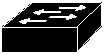
\includegraphics{switch.pdf}};
                            \node[onslide=<2->{white,opacity=0}] at (0,-0.6){B:1};
                            \node[onslide=<1>{white,opacity=0}] at (0,-0.6){B:3};
                        \end{tikzpicture}
                    }
                };

                \draw
                (A) -- (C)
                (C) -- (D)
                (B) -- (D)
                (D) -- (client);

                \draw [red, thick, dashed, onslide=<2->{white}]
                (A) -- (B);
            \end{tikzpicture}
        \end{figure}
    \end{minipage}%
    \begin{minipage}{.5\textwidth}
        \begin{enumerate}[<+(2)->]
            \item Vergleiche alle Bridges mit allen anderen
            \item Entferne Duplikate mit höherer Message Age
        \end{enumerate}
        \pause
        Dadurch bleiben alle korrekten Annahmen erhalten
    \end{minipage}
\end{frame}

\begin{frame}{Visualisierung}
    \centering
    \begin{tikzpicture}[]
        \node[white,onslide=<2->{black}] (0) at (7.000000,20) {Root};
        \node[white,onslide=<3->{black}] (1) at (2.333333,18) {A};
        \node[white,onslide=<4->{black}] (3) at (7.000000,18) {B};
        \node[white,onslide=<5->{black}] (4) at (11.666667,18) {};
        \node[white,onslide=<6->{black}] (2) at (11.666667,16) {C};

        \draw[white,onslide=<8->{black}] (0) -- (1);
        \draw[white,onslide=<8->{black}] (0) -- (3);
        \draw[white,onslide=<8->{black}] (0) -- (4);
        \draw[white,onslide=<7->{black}] (4) -- (2);
    \end{tikzpicture}
\end{frame}

\begin{frame}{Überblick}
    \begin{itemize}
        \item \textbf{Einleitung \& Motivation}
        \item \textbf{Spanning Tree Protocol (STP)}
        \item \textbf{STPViz}
        \item \alert{\textbf{Software-Switch}}
        \item \textbf{Tests}
        \item \textbf{Zusammenfassung \& Ausblick}
    \end{itemize}
\end{frame}

\begin{frame}{Software-Switch}
    \begin{itemize}
        \item Grund
        \item Funktionsweise
        \item Grenzen \& Beschränkungen
    \end{itemize}
\end{frame}

\begin{frame}{Überblick}
    \begin{itemize}
        \item \textbf{Einleitung \& Motivation}
        \item \textbf{Spanning Tree Protocol (STP)}
        \item \textbf{STPViz}
        \item \textbf{Software-Switch}
        \item \alert{\textbf{Tests}}
        \item \textbf{Zusammenfassung \& Ausblick}
    \end{itemize}
\end{frame}

\begin{frame}{Testing}
    \begin{itemize}
        \item Setup
        \item Physisches Setup
        \item Tests
        \item Resultate
    \end{itemize}
\end{frame}

\begin{frame}{Überblick}
    \begin{itemize}
        \item \textbf{Einleitung \& Motivation}
        \item \textbf{Spanning Tree Protocol (STP)}
        \item \textbf{STPViz}
        \item \textbf{Software-Switch}
        \item \textbf{Tests}
        \item \alert{\textbf{Zusammenfassung \& Ausblick}}
    \end{itemize}
\end{frame}

\begin{frame}{Zusammenfassung und Ausblick}
    \begin{itemize}
        \item STPViz Fähigkeiten
        \item STPViz Grenzen
        \item Software-Switch
        \item Sonstige Dinge (OpenWrt, dd-wrt)
    \end{itemize}
\end{frame}

\begin{frame}{Message}
Ich hätte gerne, dass Zuseher folgendes mit nach Hause nehmen:\\
\begin{itemize}
    \item Information aus STP zu extrahieren ist schwer, da es nur lokales Wissen benutzt.
    \item Wir haben es trotzdem geschafft (nur halt nicht mit maximaler Informationsdichte).
    \item Es gibt nicht viele Use Cases, aber es gibt sie.
    \item STPViz ist eine gute Grundlage für weitere Arbeiten.
\end{itemize}
\end{frame}

\end{document}
